\section{Tracks}
\label{chp:obj:trk}

The solenoidal magnetic field of the ID bends charged particles in the transverse plane along an helicoidal trajectory with a radius of inversely proportional to its momentum. When charged particles traverse sensitive detector elements of the ID, they deposit energy through ionisation. These energy deposits are read out as hits, which are used to form space points. Each Pixel hit corresponds to one space point, while SCT space points are formed from pairs of SCT hits from each side of a module.
Tracks are the reconstruction of these trajectories from the space points. Therefore, tracks enter at multiple levels in the definition of the physics objects used for physics analyses: from the reconstruction of electrons and muons, to the calculation of lepton isolation and the pileup suppression in jets, as well as reconstruction of decays of long-lived particles such as $b$-hadrons.
In a nutshell, track reconstruction can be divided into the procedure of finding track candidates, the pattern recognition, and the estimation of the parameters that describe the particle trajectory, the track fit \cite{Cornelissen:1020106}.\par
The reconstruction of tracks in the ID involves several algorithms. The main sequence is referred to as ``inside-out'' track finding, which consists of the following steps:

\bi
\ib  Track finding starts with the formation of space point triplets (seeds).
\ib  Seeds that pass the initial requirements are then input to a track-finding algorithm that attempts to complete the track candidates within the silicon detector combining space points.
\ib Ambiguities in track candidates are solved eliminating track candidates from random hit combinations or track duplicates. 
\ib Track candidates passing the previous stage are extended outward to the TRT if they are within the TRT coverage.
\ei

\noindent For signals in the TRT that are not associated to any track candidate by the inside-out reconstruction, a second algorithm, referred to as ``outside-in'', is applied in order to reconstruct tracks from secondary charged particles. The algorithm uses as seeds hits in the TRT and extrapolates to the silicon detector.
Several optimisations of the track reconstruction were added for Run 2, from improvements to the seed purity, to an update of the ambiguity-solving method in dense environments \cite{ATL-PHYS-PUB-2015-006}.\par
A reconstructed track is characterised by the following set of parameters (see figure \ref{sec:trk:fig:par}): $(d_{0},z_{0}, \phi, \theta, q/p )$, where
$d_{0}$ and $z_{0}$ stand for the track impact parameters in the transverse and longitudinal planes respectively, $\phi$ and $\theta$ denote the azimuthal and polar angle respectively, and $q/p$ represents the charge over momentum. The impact parameters are often expressed with respect to the reconstructed hard-scatter primary vertex in the event.

\bfig[htb!]
\centering
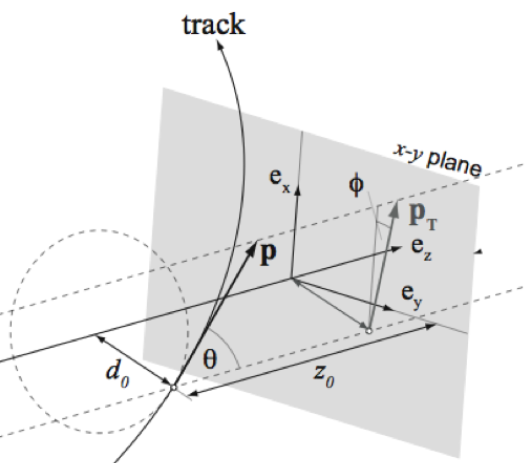
\includegraphics[width=0.4\textwidth]{figures/Objects/trackparameters.png}
\captionsetup{width=0.85\textwidth} \caption{\small Illustration of the geometric definition of the track parameters.}
\label{sec:trk:fig:par}
\efig

The track reconstruction efficiency $\epsilon_{\rm trk}$, determined from the simulation, is parametrised in two-dimensional bins of $\pt$ and $\eta$ and
is defined as:

\be
\epsilon_{\rm trk}(\pt,\eta)=\frac{N_{\rm rec}^{\rm matched}(\pt,\eta)}{N_{\rm gen}(\pt,\eta)},
\ee

\noindent where $N_{\rm rec}^{\rm matched}(\pt,\eta)$  is the number of reconstructed tracks matched to a generated primary charged particle and $N_{\rm gen}(\pt,\eta)$ is the number of generated primary charged particles in that bin. A track is matched to a generated particle if the weighted fraction of hits on the track that originate from that particle exceeds $50\%$.
Figure \ref{sec:obj:fig:efftrk} presents the track reconstruction efficiency estimated in simulated events with at least one charged particle with $\pt >500$ $\mev$ and $|\eta|<2.5$. The efficiency raises with $\pt$  and it flattens out, reaching a value as high as $\approx 90\%$ for tracks with $\pt>5$ GeV. As a function of $\eta$, the efficiency averaged over $\pt$ reaches $\approx 90\%$ in the central region and drops below $75\%$ in the forward region. 

\begin{figure}[h!]
\begin{subfigure}{0.5\textwidth}
  \centering
  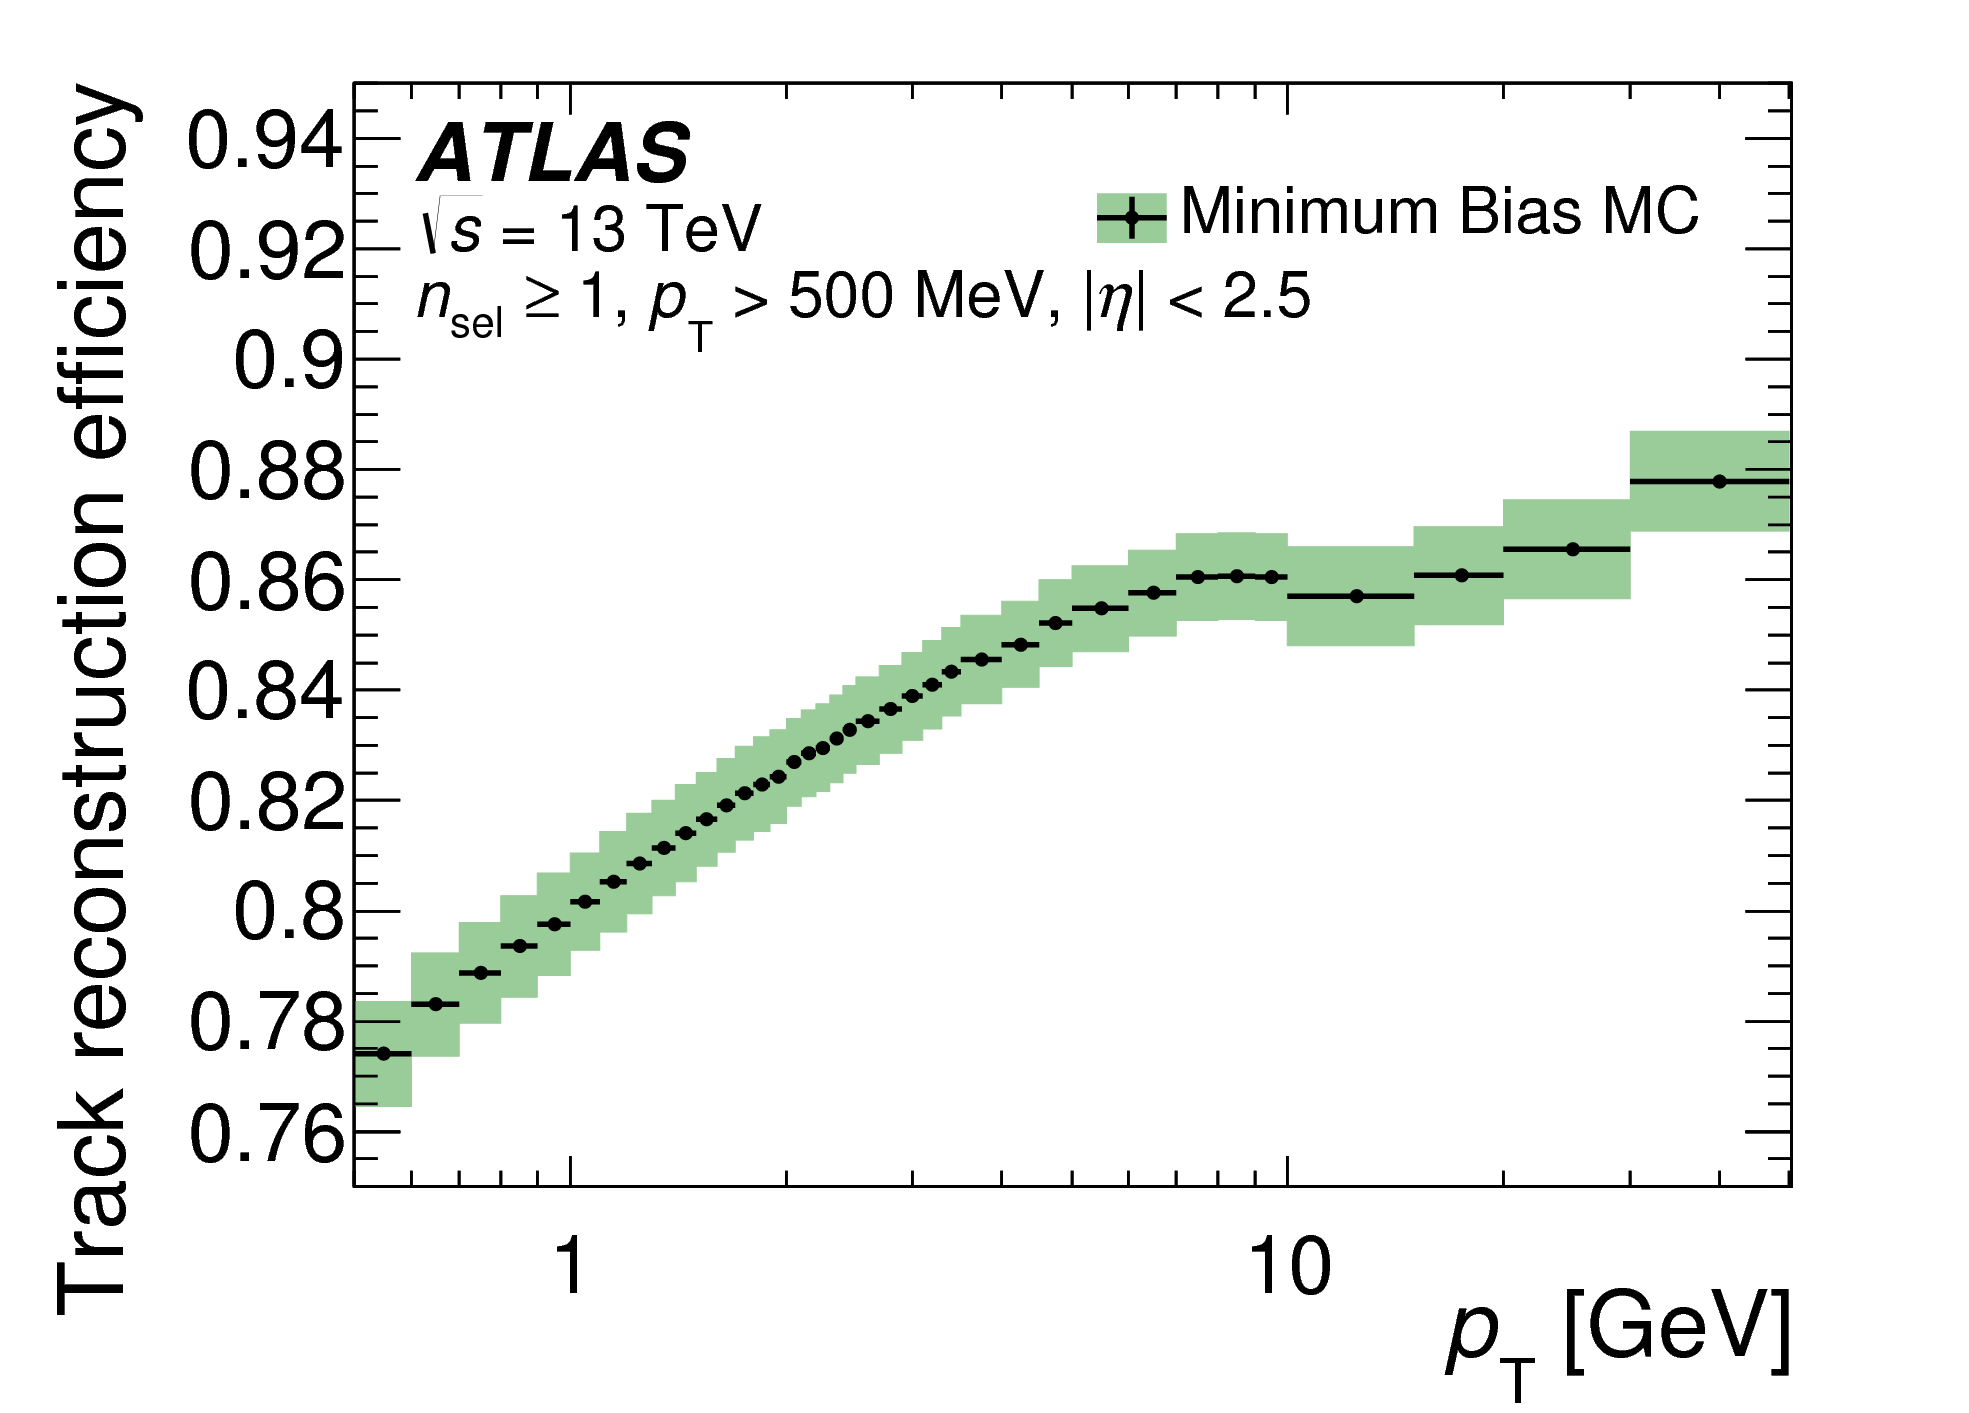
\includegraphics[width=0.9\textwidth]{figures/Objects/efftrkpt.png}
  \caption{}
  \label{sec:obj:fig:efftrkpt}
\end{subfigure}
\begin{subfigure}{0.5\textwidth}
  \centering
  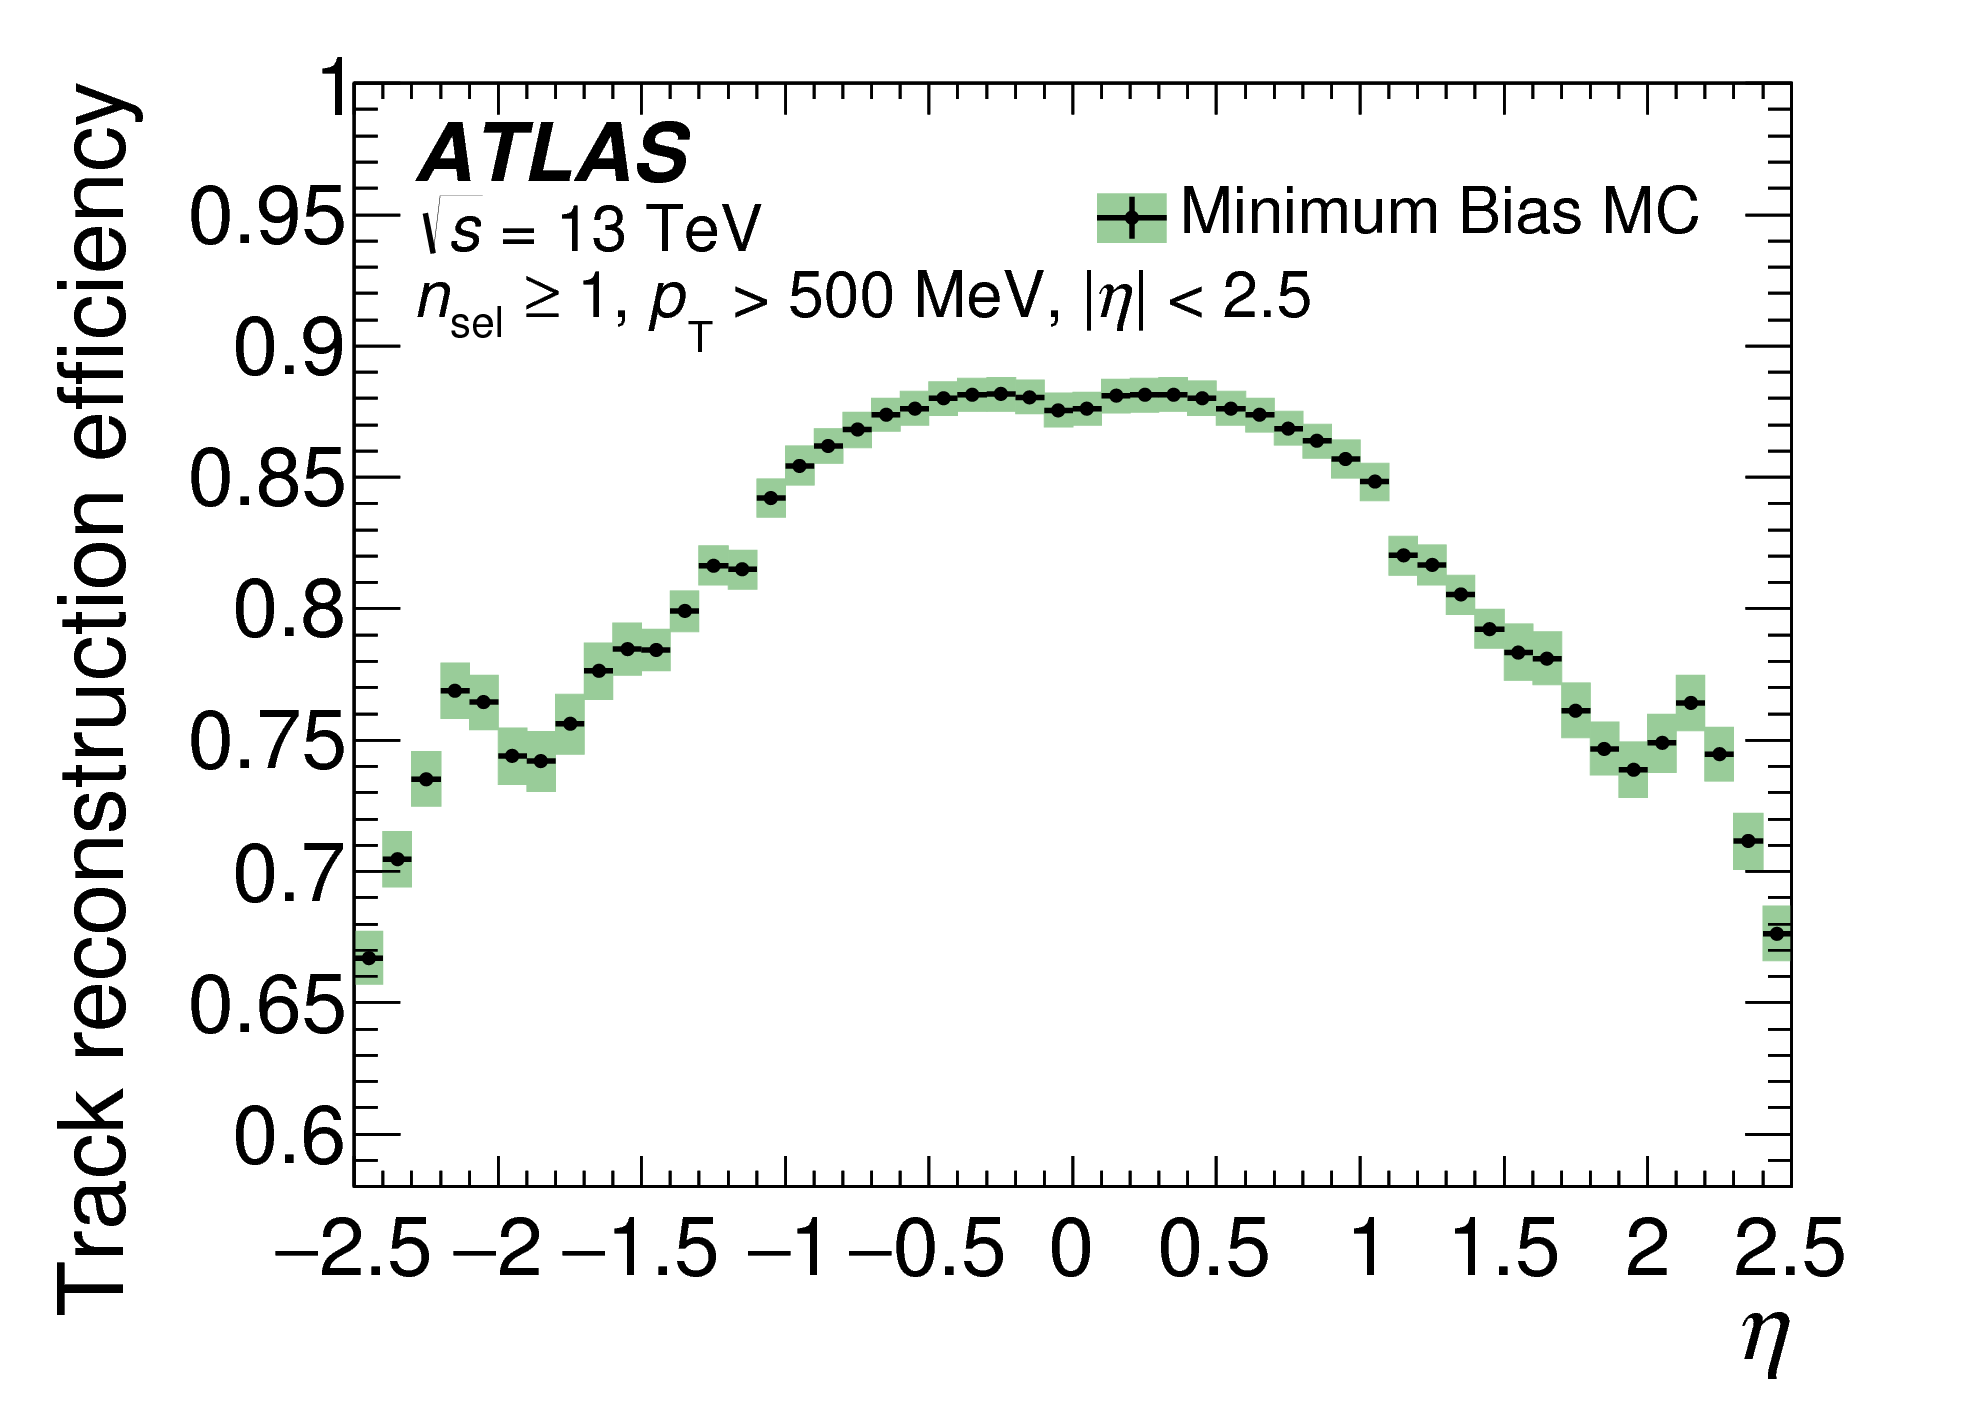
\includegraphics[width=0.9\textwidth]{figures/Objects/efftrketa.png}
  \caption{}
  \label{sec:obj:fig:efftrketa}
\end{subfigure}

\captionsetup{width=0.85\textwidth} \caption{\small The track reconstruction efficiency as a function of (a) $\pt$ and (b) $\eta$ as estimated in simulated minimum bias events. The statistical uncertainties are shown as black vertical bars, the combination of statistical and systematic uncertainties as green shaded areas. From reference \cite{Aad:2016mok}.}
\label{sec:obj:fig:efftrk}
\end{figure}




